\documentclass[11pt]{article}
\usepackage[a4paper,total={6in,8in},margin=1in]{geometry}
\usepackage[utf8]{inputenc} % allow utf-8 input
\usepackage[T1]{fontenc}    % use 8-bit T1 fonts
\usepackage{microtype,inconsolata}
\usepackage{times,latexsym}
\usepackage{graphicx} \graphicspath{{figures/}}
\usepackage{amsmath,amssymb,mathabx,mathtools,amsthm,nicefrac}
\usepackage[linesnumbered,ruled,vlined]{algorithm2e}
\usepackage{enumitem}
\usepackage[pagebackref,breaklinks,colorlinks]{hyperref}
\usepackage[skip=3pt,font=small]{subcaption}
\usepackage[skip=3pt,font=small]{caption}
\usepackage[dvipsnames,svgnames,x11names,table]{xcolor}
\usepackage[capitalise,noabbrev,nameinlink]{cleveref}
\usepackage{booktabs,tabularx,colortbl,multirow,multicol,array,makecell,tabularray}
\usepackage[english]{babel}
\definecolor{color-C00000}{rgb}{0.75,0,0}
\definecolor{red}{rgb}{1,0,0}
% \usepackage{upgreek}

\begin{document}
{\centering \textbf{Computer Vision I : Project \#3} (15 points)\par} 


\textbf{This project is} \textbf{\textcolor{color-C00000}{extremely}} \textbf{hard and time consuming. For reference: a properly written code would take roughly 16 hours to finish running on a 5-year-old Mac Pro.} \textbf{\textcolor{color-C00000}{START EARLY!}} 

\section{Background} 

This project is based on Chapter 3: Textures. You shall read the textbook and understand the underlying logistics before writing your code.

\subsection{Python Library}

Please install the latest cv2, PIL, numpy, scipy, matplotlib, tqdm, torch (including torch-vision), and the cython (if you want) packages. 
\color{black}

\subsection{What to hand in?}

Please submit both a formal report and the accompanying code. For the report, kindly provide a PDF version. You may opt to compose a new report or complete the designated sections within this document, as can be started by simply loading the tex file to Overleaf. Your score will be based on the quality of \textbf{your results}, \textbf{the analysis} (diagnostics of issues and comparisons) of these results in your report, and your \textbf{code implementation}. You may delete all the images before handing them in, as they may be too large for the autograder.

\paragraph{Notice}
1) Do not modify the function names, parameters, and returns in the given code, unless explicitly specified in this document. 2) The \textbf{maximum score} of the autograder demonstrated is $4.5$, another $0.5$ will leave for deeper evaluation. 

\subsection{Help}

Make a diligent effort to independently address any encountered issues, and in cases where challenges exceed your capabilities, do not hesitate to seek assistance! Collaboration with your peers is permitted, but it is crucial that you refrain from directly \textcolor{red}{examining or copying one another's code.}  Please be aware that you'll fail the course if our \textbf{code similarity checker}, which has found some prohibited behaviors for Project 2, detects these violations.

For details, please refer to \url{https://yzhu.io/s/teaching/plagiarism/}

\clearpage

\section{Self-check Questions}

\textbf{You may skip these questions}, as the questions below are just some help for accomplishing the project. You don't need to answer them in your report, and the correct answers to the questions should be explored by yourself. 
\begin{enumerate}
    \item Why is the FRAME model structured in the manner delineated within the referenced literature?
    \item What is the definition of ``sweep'' in the FRAME model?
    \item How to calculate the distance (difference) of two histograms within the framework of the FRAME model?
    \item Why does the FRAME model work? What does the learning process minimize?
    \item What is the operational mechanism of the Gibbs Sampler within the FRAME model?
    \item What is the learning mechanism of the Julesz Ensemble?
    \item What is the relationship between the Julesz Ensemble and the FRAME model?
\end{enumerate}
\section{Questions To Answer}
\textbf{You should answer the following questions in your report.} Please copy the questions in your report and answer \textbf{briefly} with no more than 5 sentences. 

\noindent\textit{Hint: It's recommended to finish the coding part before answering the questions.} 
\begin{enumerate}
    \item What is the definition of Julesz Ensemble?
    
    \textbf{Answer:}\ The Julesz Ensemble is a set of images with identical statistical properties, introduced by psychologist Bela Julesz to study human visual perception of textures.

    \item Why is the histogram tail important in synthesis?
    
    \textbf{Answer:}\ Because it captures the distribution of the less frequent but often significant high or low values in the data.

    \item Do I need to perform convolution on the whole image while performing gibbs sampling for a single pixel?

    \textbf{Answer:}\ Yes, it's required to do so for the whole histogram.

    \item In the code, what is the recommended method to generate the value of a pixel given the distribution of $p(val|I_{-s})$?

    \textbf{Answer:}\ By using the filter with greatest error.

    \item How is the conditional probability $p(I_s = val|I_{-s})$ computed within the Gibbs Sampler?

    \textbf{Answer:}\ By computing the difference between filtered synthesis image and filtered original image.

    \item Is the FRAME model guaranteed to converge? Why and why not? (\textit{Hint: Read Chapter 9})

    \textbf{Answer:}\ No, it's not. there is no guarantee of convergence without specific conditions and parameters being met.

    \item How to update $\lambda$ in the FRAME model?

    \textbf{Answer:}\ By finding the maximum of L.

    \item How to select new filters within the FRAME model?

    \textbf{Answer:}\ By maximizing the K-L divergence.
\end{enumerate}

\clearpage

\section{Part 1: Julesz Ensemble}

\paragraph{Objective}

This part explores the minimax entropy learning procedure for texture modeling and synthesis. We'll study its capability and limitations. The figure below depicts 3 texture examples included in the zip file.

\begin{figure}[ht!]
    \centering
    \hfill%
    \begin{subfigure}[]{0.333\linewidth}
        \centering
        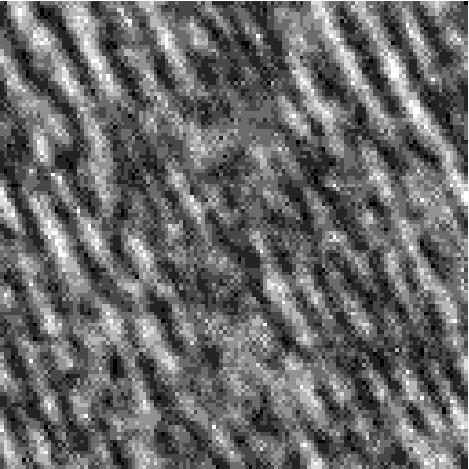
\includegraphics[width=\linewidth]{figs_for_latex_only/image1.jpg}
        \caption{fur}
    \end{subfigure}%
    \hfill%
    \begin{subfigure}[]{0.333\linewidth}
        \centering
        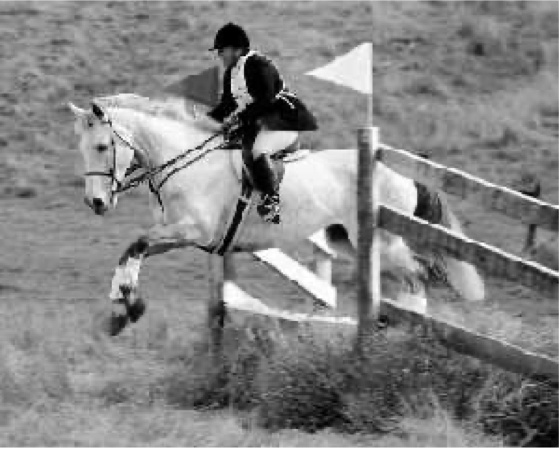
\includegraphics[width=\linewidth]{figs_for_latex_only/image2.jpg}
        \caption{horse}
    \end{subfigure}%
    \hfill%
    \begin{subfigure}[]{0.333\linewidth}
        \centering
        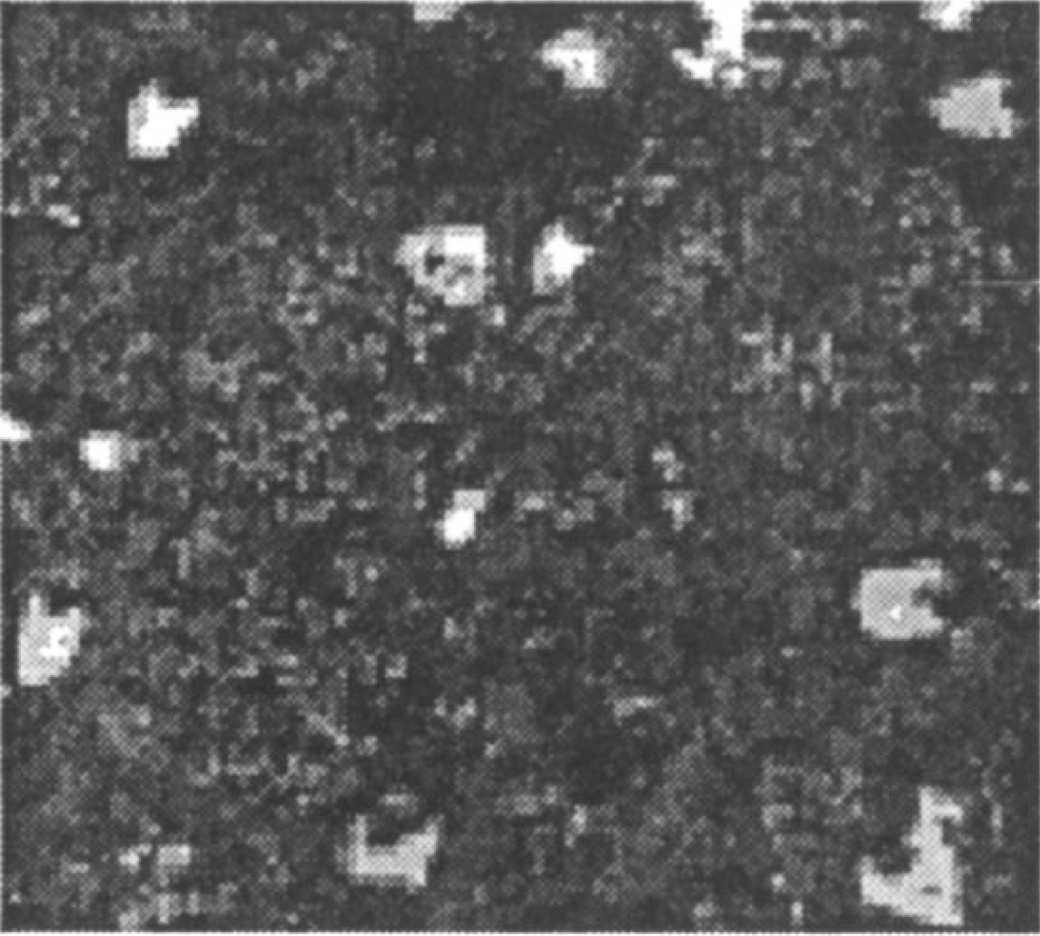
\includegraphics[width=\linewidth]{figs_for_latex_only/image3.jpg}
        \caption{mud}
    \end{subfigure}%
\end{figure}

\subsection{Experiment}

For each input image, select a set of filters and extract the histograms of filter responses. We define the Julesz ensemble as the images that reproduce the observed histograms based on the chosen filters. The synthesis process commences with a noise image generated from a uniform distribution and progresses until it aligns with all the selected histograms. Specifically, the procedure continues to select additional filters until the filtered histograms match within a defined epsilon error. To achieve this, a Gibbs sampler with an annealing scheme is employed. 

To mitigate computational complexity, it is suggested to synthesize the image in 8 gray levels {[}0,7{]} (don't forget to rescale back!) with a size of 64x64 pixels (128x128 is also okay, but it will take more time). The \textbf{torus boundary condition} addresses boundary effects. It is noteworthy that the primary focus should be on closely matching histograms at the tail bins. This involves assigning specific weights to the 15 bins, such as {[8, 7, 6, 5, 4, 3, 2, 1, 2, 3, 4, 5, 6, 7, 8]} (just an example!).

\subsection{Instructions}

\subsubsection{Overview}\label{subsubsec:overview}

The following is an overview procedure of the project:

1) Generate a filter bank by ``filters.py.''

2) The set of chosen filters S is initially empty.

3) Randomly sample a synthesized image I (sample the intensity of each pixel uniformly from {[}0,7{]}).

4) For each unselected filter, calculate its response histogram on both the input image and the currently synthesized image I. Ensure that the bin range of the histogram corresponds to the minimum and maximum response values of the input image. Subsequently, compute the \textcolor{red}{weighted difference (error)} between the two histograms.

5) If the highest error is smaller than a threshold, go to step 8. Otherwise, choose the filter with the highest error and add it to the chosen set S.

6) Use the Gibbs function to sample a new image I', and replace I with I'. (Hint: the input of the Gibbs function includes the synthesized image I from the last iteration, chosen filters set S, histograms of chosen filters' responses on the input image, and the corresponding bin ranges of the histograms.)

7) Compute the total error between the new I and the input image based on the new set S. This is the error you must show for the report. Then, go to step 4.

8) Output the synthesized image I as the final result.

\subsubsection{Details}

\begin{enumerate}
    \item ``filters.py'' contains a Python function ``get\_filters()'', which generates a set of filters in the format of matrices. 
    \textbf{Guidance}:
    \begin{itemize}
        \item You need to add more filters. For instance, you should at least add the Dirac delta function whose response is the intensity of a given pixel.\label{mark-A.}
    \end{itemize}
    \item  ``julesz.py'' contains a function ``get\_histogram()'', which computes the \textcolor{red}{normalized} filter response histogram on an image. 
    \textbf{Guidance:}  
    \begin{itemize}
        \item You should fill in the ``conv()'' function and the ``get\_histogram()'' function. 
        \item Noticed that the ``conv()'' function returns the image's filtered response which holds the \textbf{\textcolor{red}{same shape}} as the input image. Therefore, you should consider carefully the padding method.
        \item The ``get\_histogram()'' function should be designed to allow the specification of the bin range, which corresponds to the maximum and minimum responses of the filter on the input image when computing the histogram. Note that the output histogram should be normalized by (image height) * (image width). Therefore, you need to multiply the normalized histograms by (image height) * (image width) to compute the difference (error) between two histograms.
        \item Note that when calculating the histogram of each filtered response, you should use the same bin range for both the input image and the synthesized image.
    \end{itemize}
    \item \textbf{In this step, you can modify the ``gibbs.py'' file (including deleting all the codes and changing the file name).} We present two approaches for implementing the Gibbs sampling process: (1) Python Style (Roughly 3 hours per image with $64 \times 64$ size, Recommended) and (2) C Style (much faster).
    \textbf{Python Style (Recommended):}
    ``gibbs.py'' contains a function ``gibbs\_sample()'', which implements a Gibbs sampling process for the image synthesis. 
    \textbf{Guidance }:

    \textbf{Python Style: }
    \begin{enumerate}
        \item ``gibbs\_sample()'' is a function that sweeps the image, and there is a function ``pos\_gibbs\_sample\_update()'' which handles a single pixel of the image.
        \item In ``pos\_gibbs\_sample\_update()'', be careful while coding the process of calculating the conditional probability. (Hint: It's considerably faster to modify the specific bin responses in the existing histogram rather than performing convolution on the entire image and creating a new histogram from scratch.)
        \item When computing the histograms of the input image and the synthesized image, you must use the same bin range. For this, you may compute the maximum and minimum responses of the response of a filter on the input image, and then divide the range equally to obtain the interval of each bin. Use these bin ranges for both input and synthesized images.
        \item Assign different weights to the bins when you calculate the difference between two histograms, e.g. \texttt{abs(hists\_syn{[}x{]} - hists\_ori{[}x{]}) * w{[}x{]}}. Next, leverage the weighted difference to calculate the ``energy'' of the annealing process.
        \item Tune the coefficient of the simulated annealing process to improve the synthesis.
        \item Noticed that in the book, the selection of the location to be updated follows a uniform distribution. However, in this context, the locations may be chosen sequentially, such as following the order of \texttt{(0,0), (0,1), (0,2), $\ldots$, (0, img\_width-1), (1,0), $\ldots$}.
        \item If you have no idea, it is recommended to read section 3 of the paper ``\textit{Exploring Texture Ensembles by Efficient Markov Chain Monte Carlo- Towards a ``Trichromacy'' Theory of Texture}'' by \textit{Song-Chun Zhu, Xiu Wen Liu, Ying Nian Wu.} 
        \item \textbf{Speed Up Tips} 
        \begin{enumerate}
            \item If your implementation is done by using Torch, it'll be much faster to change to numpy.
            \item Use the \textbf{cython} library! Please first read the \href{https://cython.readthedocs.io/en/latest/src/tutorial/cython_tutorial.html}{basic tutorial}, and understand some basic logistics of \textbf{cython}. Please be cautious that the \textbf{``pyximport'' method} is the \textbf{preferred approach} as opposed to the \textbf{``setup.py'' method}. The latter may generate different files on different operating systems, and therefore please use the \textbf{``pyximport'' method} . Now, you are almost ready to speed up your Gibbs sampling, please read the \href{https://cython.readthedocs.io/en/latest/src/tutorial/numpy.html}{working with numpy} section of the document. You have done a great job, and please speed up your Gibbs sampling process with Cython!
        \end{enumerate}
    \end{enumerate}
    \textbf{C Style:}
    Sorry that we do not have a hint code for C-style. If you feel that Python is not enough you can try to study the \href{https://docs.python.org/3/library/ctypes.html}{\textbf{ctypes}} library and implement the algorithm in C. It is a much harder way and you may get crazy with ``segmentation fault,'' but you'll be much faster than Python and I believe you'll learn a lot!

    
    \textbf{Make sure that your code can be run with ``python julesz.py'' for autograding!}
    \item Fill in the ``julesz()'' method of ``julesz.py'', which should include the steps described in \cref{subsubsec:overview}.

\end{enumerate}

\subsection{Submission}

\begin{enumerate}
    \item Show the input images of your program, and report their sizes.
    \item Show the set of selected filters (enlarge them to make them visible) and print the sequence of images you synthesize by increasing the filter number.
    \item  Plot the errors of the histograms of filtered responses over the iterations (after choosing a new filter).
\end{enumerate}

\paragraph{Hints for getting nice results:}
\begin{enumerate}
    \item Match the histogram closely, especially at the tails.

\item  Try other filters not in the file.
 
\item  You can debug by setting a small image size.
 
\item  It's enough to generate good images of size $64 \times 64$ by using filters of size $3 \times 3$. However, for $128 \times 128$ input images, $3 \times 3$ filters aren't enough.

\item  For the grass figure, $128 \times 128$ size will result in a more beautiful result, but we won't deduct your score for using $64 \times 64$.
\end{enumerate}
\subsection{Outcomes}
In this part, I chose the Gabor filters as my filters, and used $[8, 4, 2, 1, 2, 4, 8]$ as the weight to highlight the edge of the image.

However, since the training process is really time-consuming, I can only finished 3 iterations with 50 sweeps, the synthesized images are shown below.

\begin{figure}[ht!]
    \centering
    \hfill%
    \begin{subfigure}[]{0.333\linewidth}
        \centering
        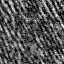
\includegraphics[width=\linewidth]{figs_for_latex_only/original.jpg}
        \caption{original}
    \end{subfigure}%
    \hfill%
    \begin{subfigure}[]{0.333\linewidth}
        \centering
        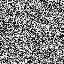
\includegraphics[width=\linewidth]{figs_for_latex_only/synthesized_0.jpg}
        \caption{synthesized1}
    \end{subfigure}%
    \hfill%
    \begin{subfigure}[]{0.333\linewidth}
        \centering
        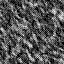
\includegraphics[width=\linewidth]{figs_for_latex_only/synthesized_2.jpg}
        \caption{synthesized2}
    \end{subfigure}%
\end{figure}

And the loss curve is shown below:
\begin{figure}[ht!]
    \centering
    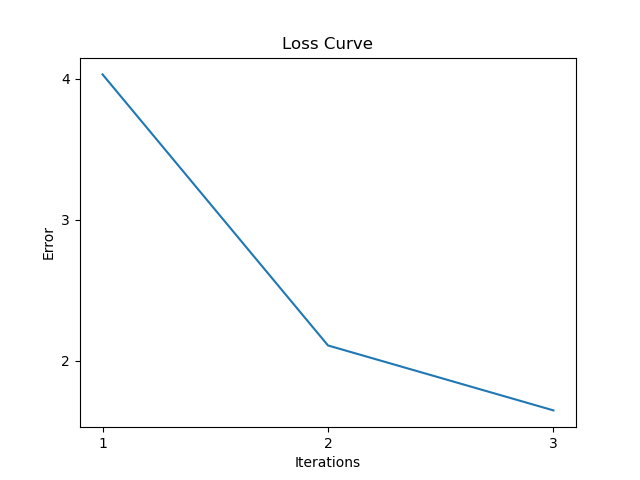
\includegraphics[width=\linewidth]{figs_for_latex_only/loss_curve.png}
    \caption{loss curve}
\end{figure}

Though the image is not totally converged, we can still see the similarity between it and the original image, showing the credibility of this method.

\section{Part 2: FRAME Model}

\textcolor{red}{Congratulations on finishing Part 1, you are marvelous!}

\subsection{Objective}

This section examines the Filters, Random Field, and Maximum Entropy (FRAME) model, which constitutes a rigorously formulated mathematical framework designed to characterize textures by integrating filtering and random field modeling. In this model, Maximum Entropy is harnessed to establish the probability distribution governing the image space, while Minimum Entropy is employed for the judicious selection of filters from a comprehensive filter bank. The amalgamation of these two facets gives rise to the overarching principle known as the ``min-max entropy principle.''

Revisiting the Principle of Maximum Entropy for constructing a probability distribution denoted as $p$ over a set of random variables, denoted as $X$, involves the following considerations. Let $\phi_{n}(x)$ denote a set of known functions such that $E_{p}\left[\phi _{n}\left(x\right)\right]=\mu _{n}$. The collection of constraints to be satisfied is denoted as $\Omega =\left\{p\left(x\right)| E_{p}\left[\phi _{n}\left(x\right)\right]=\mu _{n},\, n=1,\ldots ,N\right\}$.

The Principle of Maximum Entropy states that the choice of the probability distribution $p\in \Omega $, which maximizes the entropy $H(p)$, is a judicious one. As a consequence, this yields a solution in the form of $p\left(x;\Lambda \right)=\frac{1}{Z(\Lambda )}\exp \left\{-{\sum }_{n=1}^{N}\lambda _{n}\phi _{n}\left(x\right)\right\}$, where $\Lambda$ represents the Lagrange multipliers $\left\{\lambda _{1},\lambda _{2},\ldots ,\lambda _{N}\right\}$, and the partition function $Z\left(\Lambda \right)$ is defined as $Z\left(\Lambda \right)=\int \exp \left\{-{\sum }_{n=1}^{N}\lambda _{n}\phi _{n}\left(x\right)\right\}dx$.

From this foundational principle, the Filters, Random Fields, and Maximum Entropy (FRAME) model can be derived (see ``Computer Vision \textendash{} Statistical Models for Marr's Paradigm'' or ``Filters, Random Fields and Maximum Entropy (FRAME): Towards a Unified Theory for Texture Modeling'').

\subsection{Instructions}

To learn the FRAME model, you must select filters and learn $\Lambda$. Note that in this part, only the \textbf{\textcolor{red}{fur image of size $64 \times 64$}} is needed.
\begin{enumerate}
    \item Read the relevant chapter in the textbook.
    \item Create a copy of your codes in part 1 (``filters.py'' to ``filters\_frame.py'', ``gibbs.pyx'' to ``gibbs\_frame.pyx'').
    \item  Adjust your Gibbs sampling code to compute the term $-\sum _{n}\lambda _{n}\phi _{n}(x)$.
    \item Create a copy ``frame.py'' of ``julesz.py''. Adjust the code to define $\Lambda $ and update $\left\{\lambda _{1},\lambda _{2},\ldots ,\lambda _{N}\right\}$ by gradient ascend on $\log p(x;\Lambda )$, i.e., 
    \begin{equation*}
        \frac{d\lambda _{n}}{dt}=\frac{d\log p(x;\Lambda ) }{d\lambda _{n}}=E_{p\left(x;\Lambda \right)}\left[\phi _{n}\left(x\right)\right]-\mu _{n} , n=1,2,\ldots ,N.
    \end{equation*}
    \item Deprecate the ``weight'' item for calculating the difference (error) of 2 histograms in part 1, as it's not needed for part 2.
    \item Set the threshold of the algorithm to a reasonable scale so that the program will not take too long. As a reference, the threshold of 0.1 will take roughly 7 hours.
    \item Change the ``julesz()'' function to ``frame()'' and adjust it according to the book.
    \item Make sure that your code can be run by ``python frame.py'' for autograding!
\end{enumerate}

\subsection{Submission}

\begin{enumerate}
    \item Plot the estimated $\Lambda =\left\{\lambda _{1},\lambda _{2},\ldots ,\lambda _{N}\right\}$ over learning iterations.
    \item Show the set of selected filters and print the sequence of images that you synthesize by increasing the filter number. 
\end{enumerate}

\paragraph{Hints}

If the implementation is deemed accurate, you  are advised to wait several procedural steps in order to observe the efficacy of the FRAME model.

\end{document}